\chapter{机械臂}
\section{机械臂简介}
我们使用的机械臂是Dobot Magician E6,它具有指示灯
\begin{itemize}
	\item 蓝色快闪:机器人启动中。
	\item 蓝色常亮:机器人上电未使能状态。
	\item 绿色常亮:机器人使能状态(未运行)。
	\item 绿色慢闪:自动运行状态。
\end{itemize}
上电后等到指示灯呈蓝色常亮即可使能,使能完毕后即可运行程序。
\par 
机械臂的LAN1口IP地址、网关等参数可以手动指定,而LAN2口IP固定为192.168.200.1,因此当忘记机械臂的IP时,可以通过LAN2连接,连接成功后去通讯设置中修改LAN1的参数。
\section{树莓派连接机械臂}
将网线连接树莓派和机械臂的LAN1口,在终端中输入
\begin{lstlisting}[style=bashstyle]
	ping 192.168.5.1
\end{lstlisting}
\par
前提是机械臂的IP是192.168.5.1,树莓派的以太网IP是192.168.5.x。
如果如下图所示,说明连接失败。
\begin{figure}[H]
	\centering
	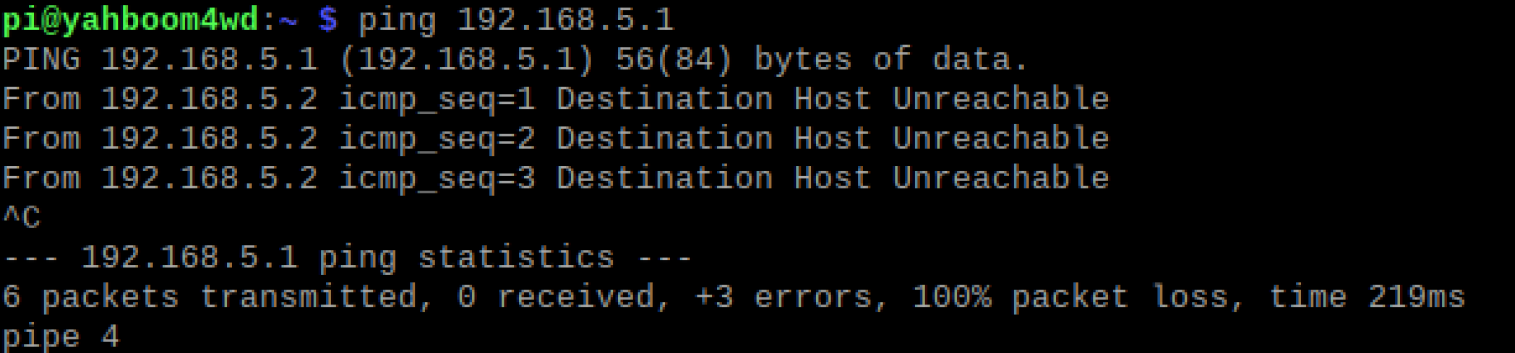
\includegraphics[width=\textwidth]{连接失败.png}
	\caption{连接失败}
	\label{fig:example}
\end{figure}
\par 
如连接失败,可等待一会再次尝试。如仍不行,解决方案还包括重启设备、插拔网线、关机静置一会等。
\begin{figure}[H]
	\centering
	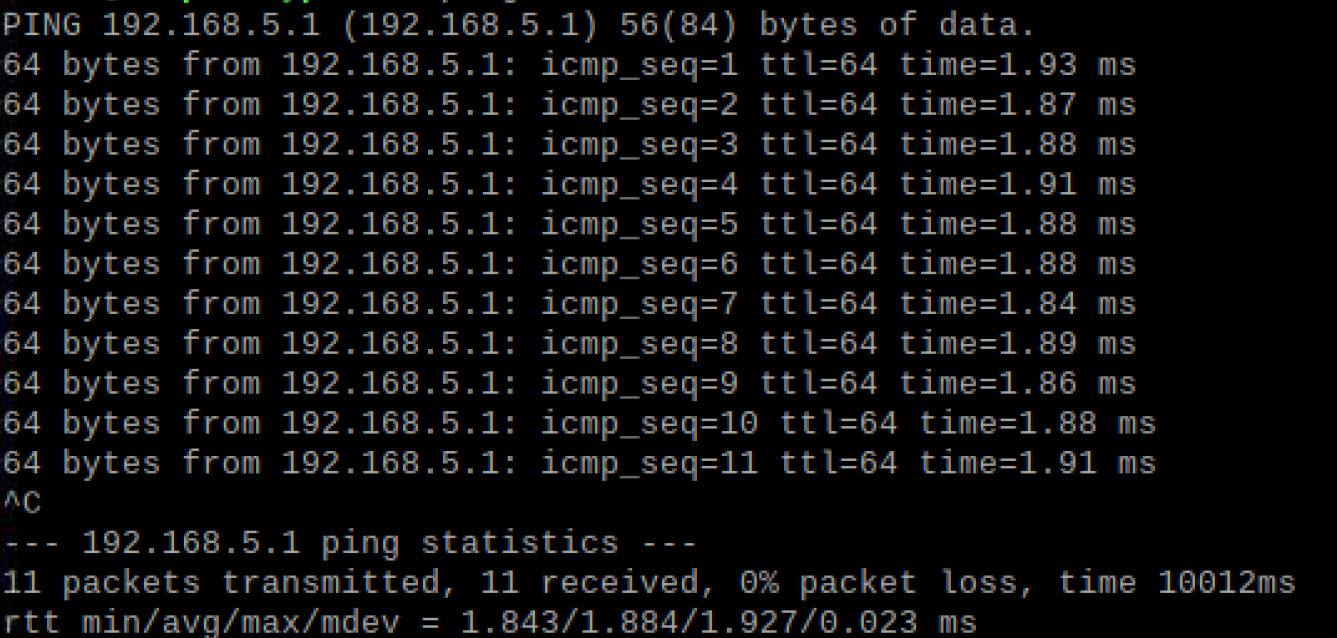
\includegraphics[width=\textwidth]{连通.png}
	\caption{连通}
	\label{fig:example}
\end{figure}
\section{机械臂脱机运行}
机械臂底部有三个按钮,从左至右分别为\textbf{电源按键}、\textbf{运行停止按键}、\textbf{使能按键}。
\par
在比赛时脱机运行,就需要\textbf{长按}运行停止按键以实现效果,但首先要在机械臂中进行相关配置。
\par
用电脑连接机械臂后,进入下图所示设置界面。
\begin{figure}[H]
	\centering
	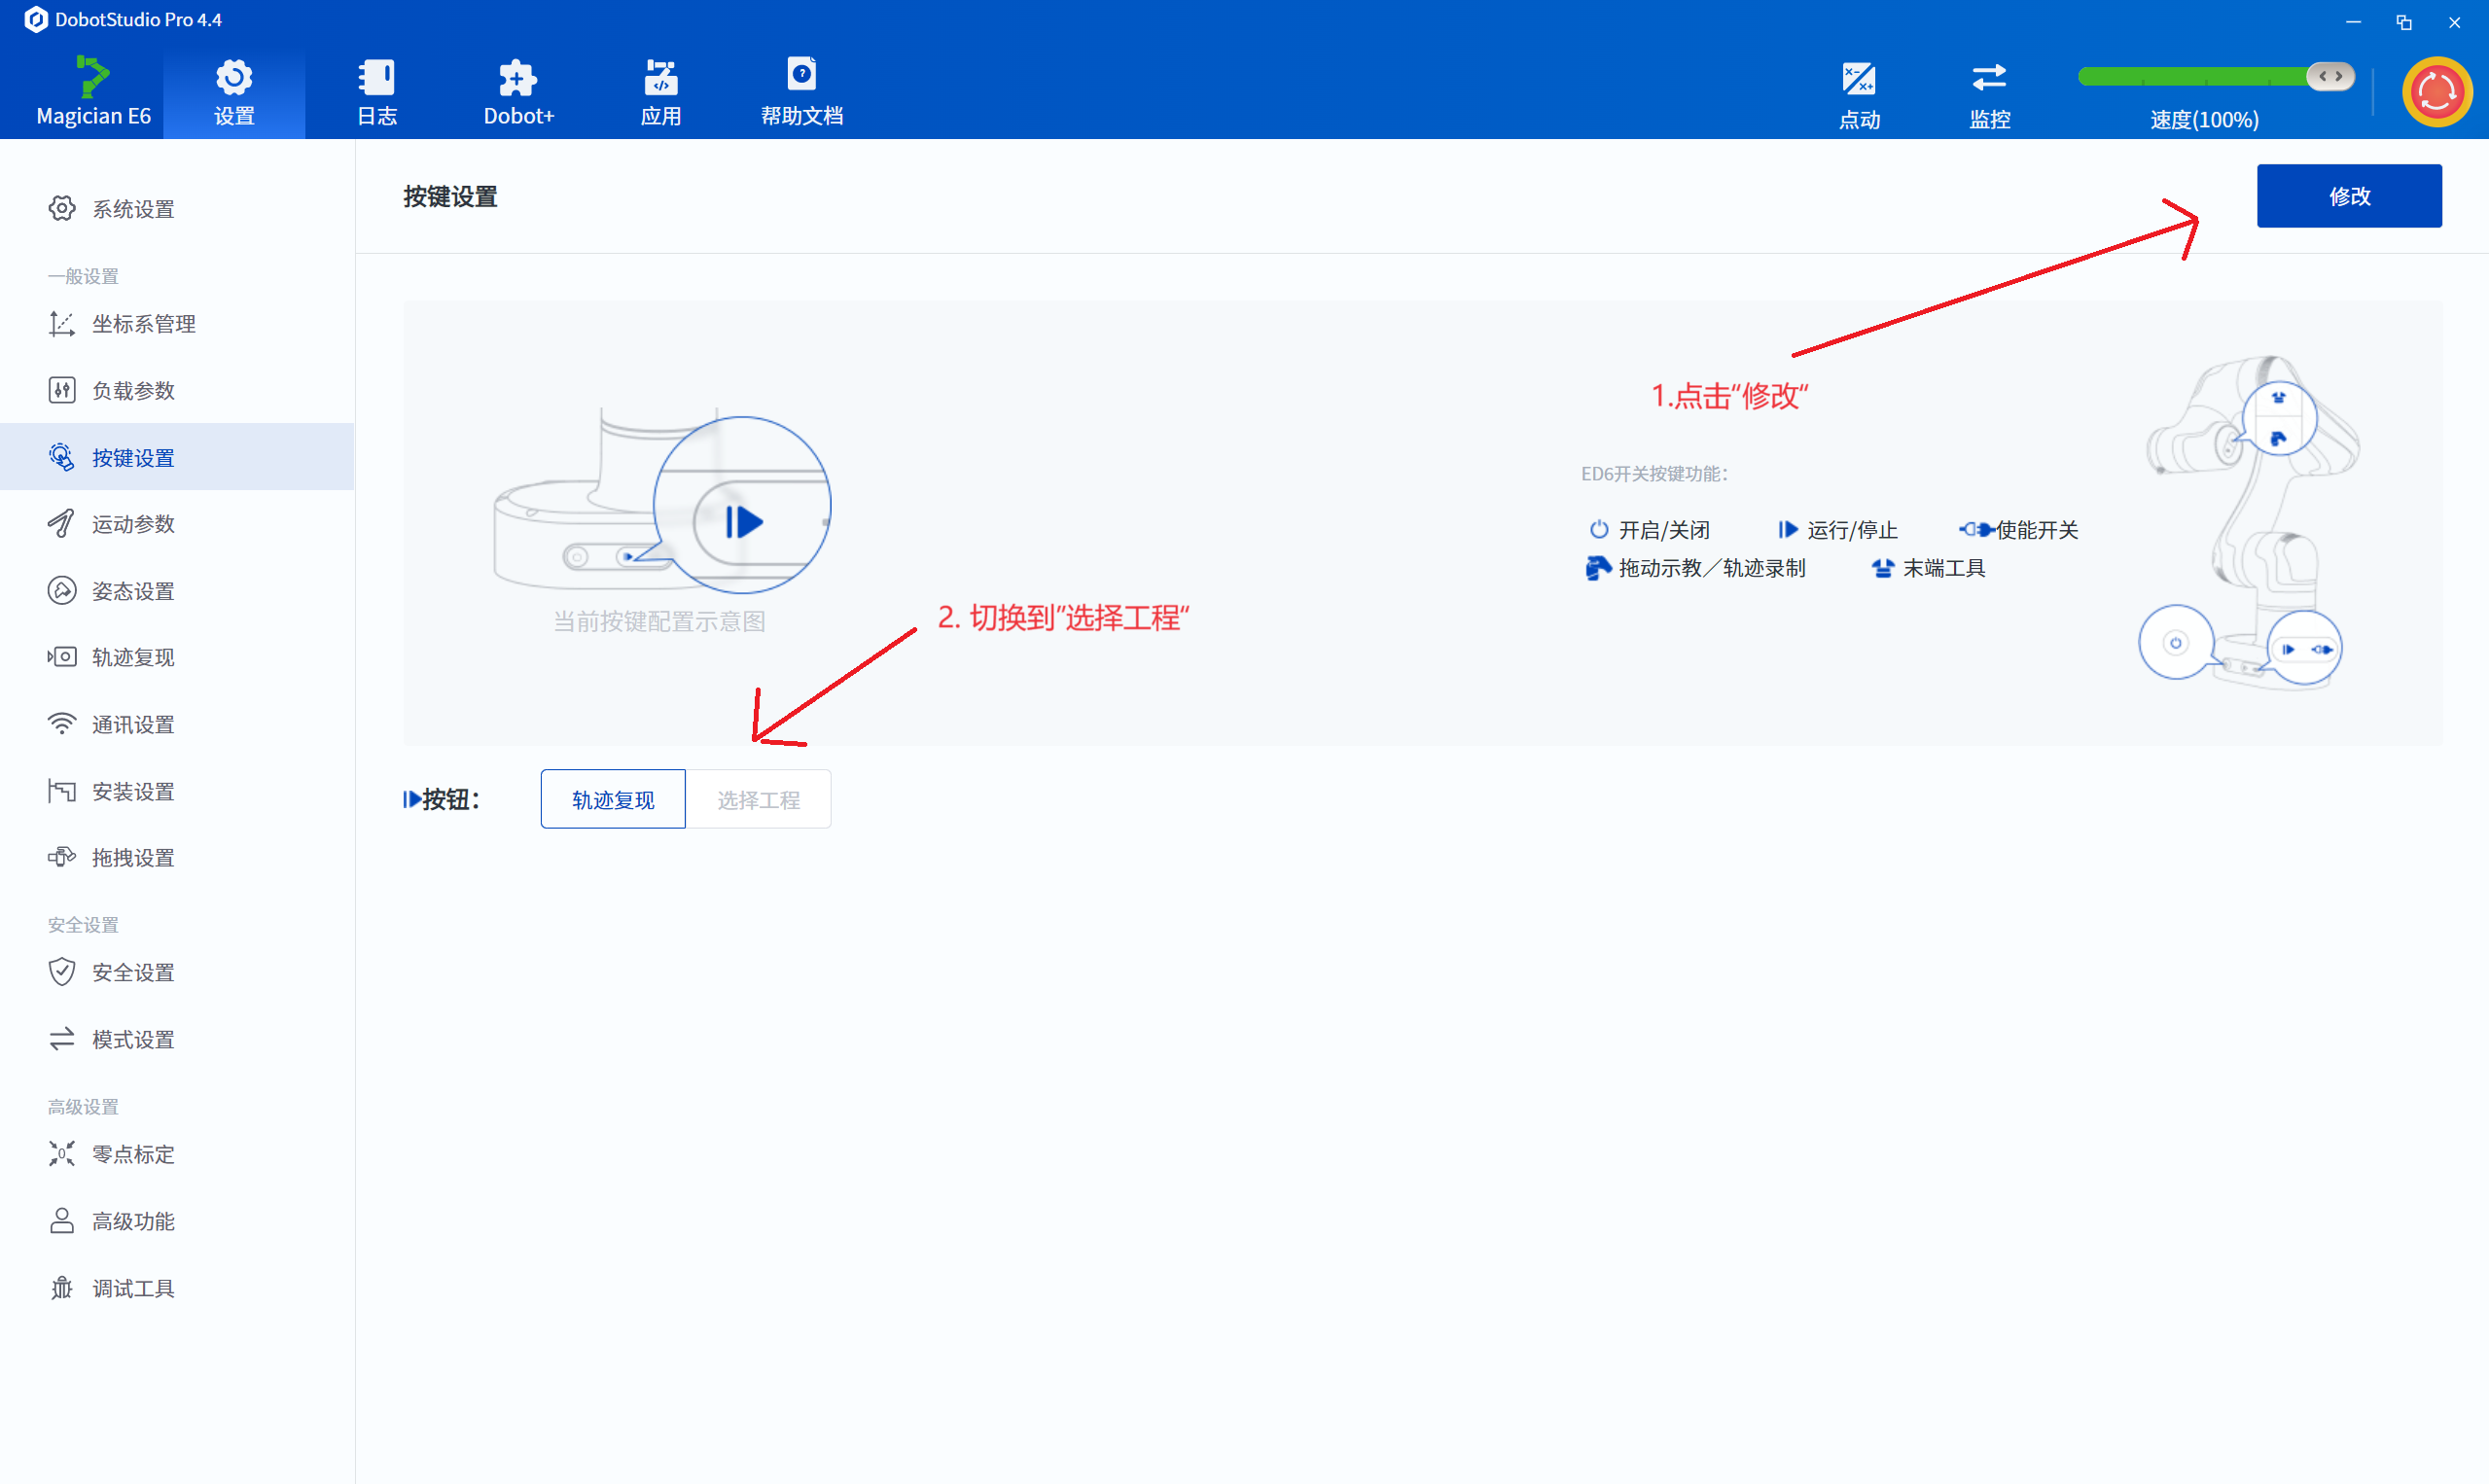
\includegraphics[width=\textwidth]{选择工程.png}
	\caption{运行停止按键设置}
	\label{fig:example}
\end{figure}
按图示操作,切换到选择工程后选择脱机后运行的工程。当然,首先要把工程保存在机械臂内。
\par
此外,中止运行则是\textbf{短按}此按键。在使能机械臂后(长按使能按键),长按运行停止按键即可启动机械臂内的工程。
\par
以下是一个例子:
\par
在机械臂内预存好以下工程
\begin{lstlisting}[style=luastyle]
	err, socket = TCPCreate(false, "192.168.5.2", 8081)
	TCPStart(socket, 20)
	while true do
		err, recBuf = TCPRead(socket, 30)
	  end
	TCPDestroy(socket)
\end{lstlisting}
\par
在树莓派中编写一个py程序socket\_test.py:
\begin{lstlisting}[style=pythonstyle]
	import socket
	import time
	sk = socket.socket(socket.AF_INET, socket.SOCK_STREAM)
	sk.bind(('192.168.5.2', 8081))
	conn, addr = sk.accept()
	sk.listen(2)
	# 打开摄像头
	while True:
		print(f'Connected to client: {addr}')
		msg = '欢迎访问服务器!' + "\r\n"
		conn.send(msg.encode('utf-8'))
		time.sleep(2)
\end{lstlisting}
\par
运行python程序后,长按机械臂的运行停止按键,观察到指示灯呈绿色且闪烁时,工程就启动了,如果能在树莓派的终端里看到大量输出,说明程序正常运行,脱机运行是可行的。
\par
注意IP地址要写成DHCP配置中的那个,同时网线连接机械臂的LAN1口。